\subsection{Performance around high-degree nodes}

Following the team's degree-stratified diagnostic, we rank nodes by degree in each seed's clean training graph. For a given $k$, we select the top $k\%$ nodes, breaking degree ties by node ID, and evaluate the original held-out test pairs with at least one endpoint in that set. The node set and test pairs remain fixed across all models and perturbations. We use $k\in\{1,5,10,20,50,100\}$, and report AUROC and AP only when the selected cohort contains both classes. All 14 conditions, seven model variants, and three seeds are retained in the accompanying CSV files; the main plots show clean and 50\% hub-priority edge deletion.

\begin{table}[H]

\centering

\small

\begin{tabular}{llccc}

\toprule

Dataset & Model & Top 5\% & Top 20\% & All nodes \\

\midrule

Cora & CN & 0.751 & 0.751 & 0.722 \\

Cora & GCN & 0.830 & 0.854 & 0.846 \\

Cora & SGDiff & 0.803 & 0.853 & 0.853 \\

\midrule

Citeseer & CN & 0.741 & 0.723 & 0.669 \\

Citeseer & GCN & 0.854 & 0.843 & 0.823 \\

Citeseer & SGDiff & 0.858 & 0.863 & 0.836 \\

\midrule

Pubmed & CN & 0.692 & 0.650 & 0.642 \\

Pubmed & GCN & 0.947 & 0.945 & 0.954 \\

Pubmed & SGDiff & 0.795 & 0.828 & 0.904 \\

\bottomrule

\end{tabular}

\caption{Clean AUROC on test pairs incident to nodes with the highest clean training degree. Values average three seeds. The 100\% column is the original full-test AUROC.}

\label{tab:topdegree}

\end{table}

\begin{figure}[H]

\centering

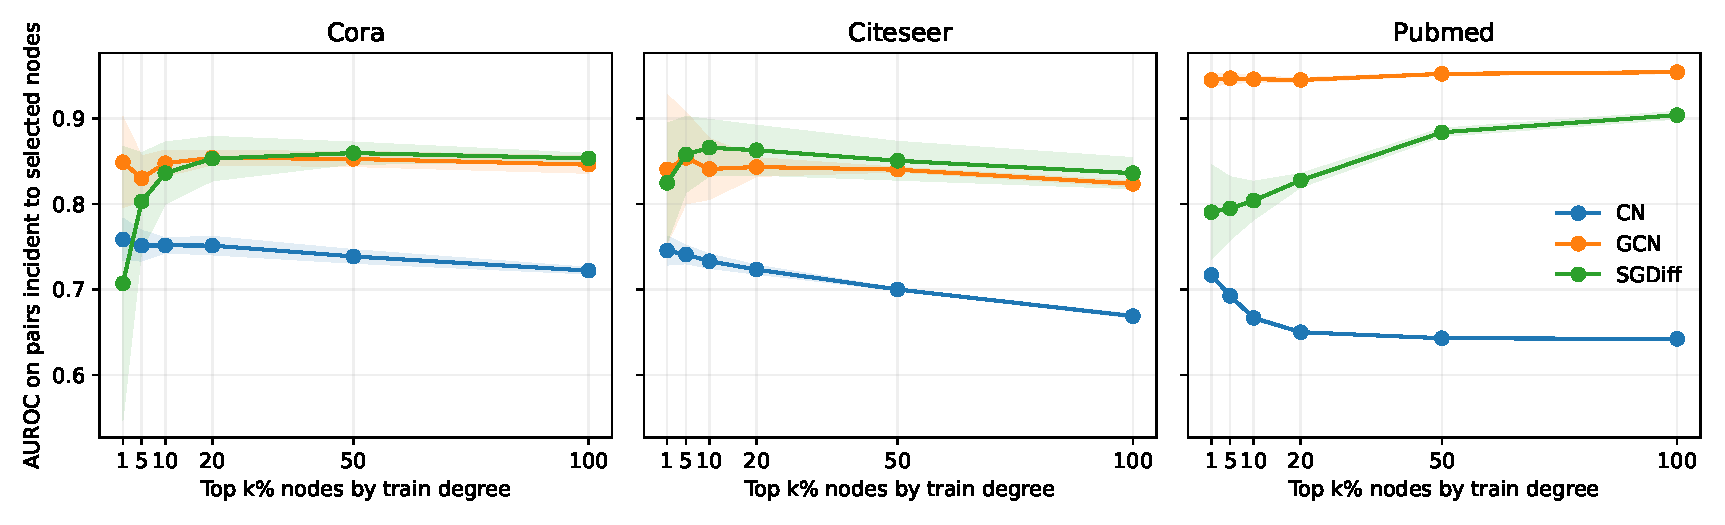
\includegraphics[width=\linewidth]{clean_top_degree_auc.pdf}

\caption{Clean AUROC as the high-degree node cohort expands. Shading shows standard deviation across three seeds.}

\label{fig:topdegreeclean}

\end{figure}

\begin{figure}[H]

\centering

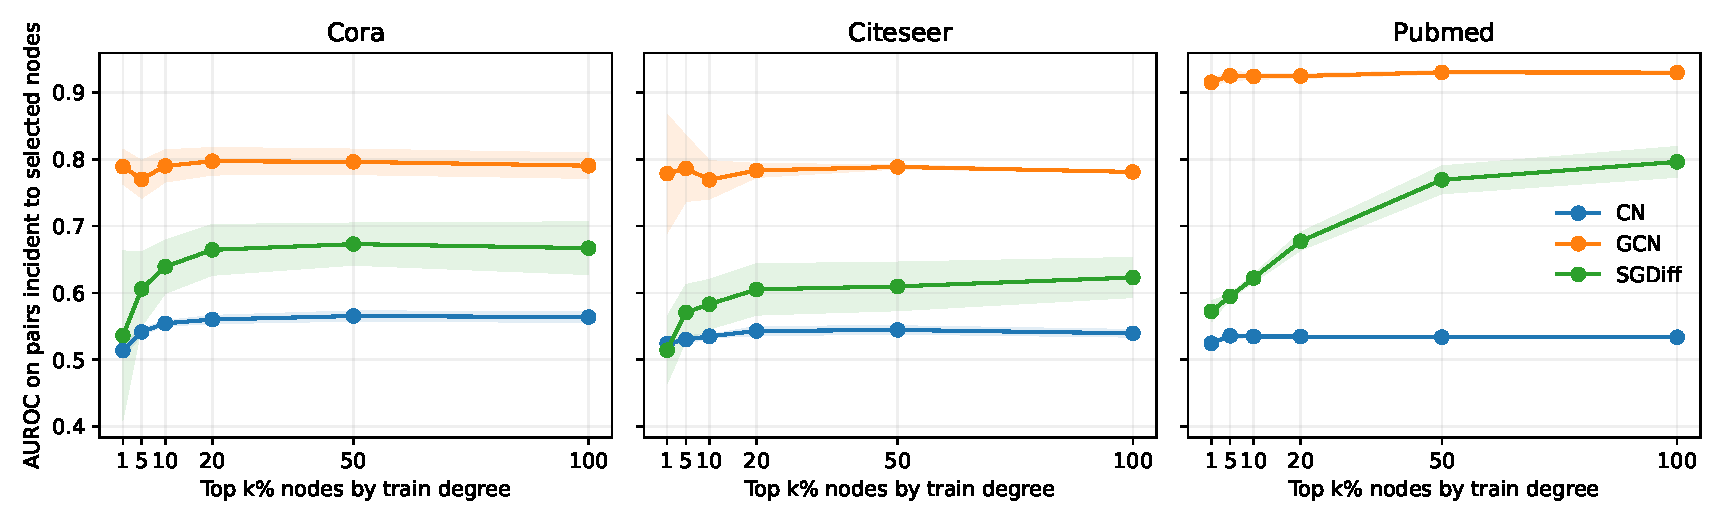
\includegraphics[width=\linewidth]{hub_delete_50_top_degree_auc.pdf}

\caption{The same fixed cohorts under 50\% hub-priority edge deletion.}

\label{fig:topdegreehubdelete}

\end{figure}

The top 1\% cohorts are highly imbalanced, especially in Cora and CiteSeer, and their curves vary substantially across seeds. Cohort AUROC is conditional on node degree; it is not the precision of the model's highest-scoring predicted links. These observations alone do not establish that SGDiff's subgraph node cap causes its hub behavior.
